\section{Results and discussion}\label{results}
This section presents the main findings of the Austrian case study. It is structured in three parts. First, Sections \ref{res_grid2030} and \ref{res_grid2040} present the Austrian gas grid in 2030 and 2040 respectively. The quantitative results for grid length, investment, and operating costs are presented for both grids. Building on this, Section \ref{res_grid_charges} focuses on the grid costs and compares the grid charges of customers today with those in 2030 and 2040. 

\subsection{Gas grid 2030}\label{res_grid2030}




\subsection{Gas grid 2040}\label{res_grid2040}

\subsection{Development of grid charges}\label{res_grid_charges}




%This section presents the most relevant results of the analyzed test bed in Vorarlberg, Austria. Section \ref{modelrun1} presents the cost-optimal gas network without an ensured supply of available gas demands (model run 1). Section \ref{modelrun2} puts focus on the (nodal) shadow prices of the cost-optimal gas network without ensured supply (model run 2). Especially, the latter highlights the impact of supplying additional gas demands at the community (or local administrative unit (LAU)) level on the network planning. Section \ref{modelrun3} shows the cost-optimal gas network with ensured supply (model run 3). Section \ref{res:com} compares total costs and shadow prices \replaced[]{with and without}{w/} ensured supply. This includes, the socialization of network costs until 2050. Finally, Section \ref{res:lum} shows the cost-optimal gas network without ensured supply under the lumpiness of gas pipelines. 
%
%\subsection{Cost-optimal gas network without an ensured supply of gas demand (CO)}\label{modelrun1}
%In this case, the planning decision is made as follows: if the network operator can treat all energy services equally and thus can decide without restrictions if gas demands are supplied or not, then the gas networks will look like those presented here. Accordingly, it is assumed that competitive alternatives without depedence on gas networks exist for each energy service need. \added[]{Note that the costs of customers not served by the network are not explicitly considered. The shadow prices (discussed in the following section) give a quantitative indication of these costs even without taking them explicitly into account.} Figure \ref{fig:1} shows an overview of the most relevant results in this case. Figure \ref{fig:1} (a) shows the high- and mid-pressure gas networks. Given the existing gas networks (see Figure \ref{fig:comparison}), it is evident that all high-pressure pipelines (in red) are refurbished. At the same time, \SI{59}{\%} of the length of mid-pressure pipelines are refurbished and \SI{41}{\%} are decommissioned. The maximum capacity of the high-pressure network level is \SI{161.92}{} and \SI{40.58}{MW} of the mid-pressure (see Figure \ref{fig:1} (b)). Figure \ref{fig:1} (c) and (d) shows the development of gas demands supplied and not supplied for both pressure/network levels. Particularly, high shares of the mid-pressure demands are covered as a result of comparable high revenues at this pressure level. At the same time, no high-pressure gas demands are covered after 2030. Note that 2030 is the assumed year of the decommissiong and refurbishment investment decision for all pipelines within the networks. 
%
%\begin{figure}[h]
%	\centering
%	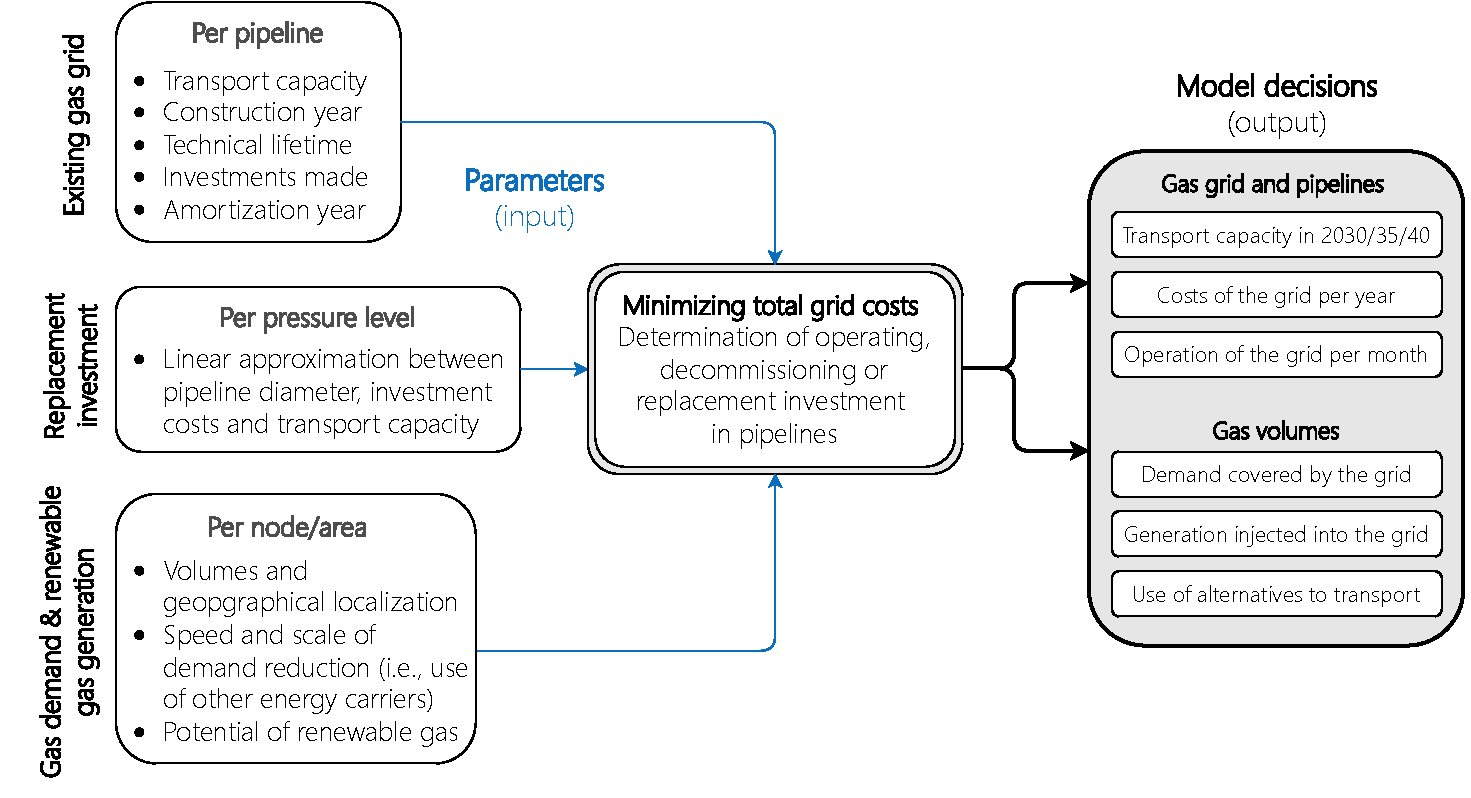
\includegraphics[width=1\linewidth]{figures/modelrun1/overview.eps}
%	\caption{Cost-optimal gas networks without ensured supply (model run 1): (a) high- and mid-pressure pipelines, (b) overview of max pipeline capacity, length, and share of decommissioned and refurbished pipeline lengths, (c) demand supplied, and (d) demand not supplied at the high- and mid-pressure network level.}
%	\label{fig:1}
%\end{figure}
%
%\subsection{Shadow prices for supplying additional gas demands of the cost-optimal gas network without an ensured supply of gas demands}\label{modelrun2}
%This section takes the cost-optimal gas network without an ensured supply of gas demands as a starting point and investigates the dual variables and shadow prices of the (nodal) gas balance constraints (see Section \ref{runs}). In this case, emphasis is put on the question: What costs arise and what network adaption is required if the network operator is required to supply an additional gas demand at the nodal level? Since the results of the previous section indicate that mid-pressure gas demands are supplied only (see particularly Figure \ref{fig:1} (c)), this section highlights (nodal) shadow prices of supplying additional gas demands at the mid-pressure network level. \added[]{The shadow prices are the dual variable of the gas demand constraint from Equation \ref{eq:notsupplied}. Here, the shadow price indicates how the value of the objective function would change if additional demand were supplied at a node. Note that these shadow prices refer to network costs only.}\vspace{0.3cm} 
%
%
%
%Figure \ref{fig:2} shows shadow prices for LAUs between 2025 and 2050. Figure \ref{fig:2} (a) shows the heatmap of the shadow prices, where the x-axis covers each year between 2025 and 2050 and the y-axis each node potentially connected to the mid-pressure network level. Thereby, each combination (i.e., node and year) is divided on the basis of four categories (i) No expansion (reduced), which means that the network is able to supply the additional gas demand without expansion and thus the objective function value is reduced by the revenues for selling the additional gas demand at the mid-pressure network level; (ii) expansion (reduced), which means that the network needs to be extended to supply the additional gas demand but the objective function value remains reduced but less than by the total revenues for selling gas demand at the mid-pressure network level; (iii) expansion (unaffected), which means that the network must be extended and the objective value is unaffected and remains constant (i.e., shadow price equal to 0), and (iv) expansion (increased), which means that the network needs to be extended and the objective value would be increased (i.e., shadow price greater than 0).
%
%\begin{figure*}[t!]
%	\centering
%	\begin{subfigure}[t]{0.5\textwidth}
%		\centering
%		\includegraphics[height=2in]{figures/modelrun2/hm_shdprice.eps}
%		\caption{Heat map/capability of the network}
%		\label{fig:2a}
%	\end{subfigure}%
%	~ 
%	\begin{subfigure}[t]{0.5\textwidth}
%		\centering
%		\includegraphics[height=2in]{figures/modelrun2/shadow_example.eps}
%		\caption{Near-feed and off-feed node}
%	\end{subfigure}
%	\caption{Shadow prices for supplying additional gas demands at the mid-pressure network level: (a) heat map identifying the capability of the gas network to supply additional mid-pressure gas demands, and (b) temporal development of the shadow price for a near-feed node (Dornbirn) and a off-feed node (Bludenz).}
%	\label{fig:2}
%\end{figure*}
%
% Figure \ref{fig:2} (b) presents the exact numbers of the shadow prices for two representative nodes, namely, a near-feed node (Dornbirn) and an off-feed node (Bludenz). Dornbirn is therefore near the gas supply/source node, and Bludenz is further away from it. The shadow price at the off-feed node has several peaks (three are marked in 2030, 2035, and 2046) and its maximum is \SI{299.2}{EUR\per MWh} in 2030. The near-feed node has two peaks (in 2030 and 2035) and its maximum is \SI{109}{EUR \per MWh} in 2030. Particularly, the development of the near-feed node after 2036 shows the capability of supplying additional gas demands since pipelines capacities are available without expansion.
%
%
%
%\subsection{Cost-optimal gas network with an ensured supply of gas demands (ES)}\label{modelrun3}
%This section shows the results in the case that the network operator should cover all gas demands within the supply area. Contrary to the previous two sections, no gas demands are not supplied. Figure \ref{fig:result2} shows an overview of the most relevant results in this case. 
%
%\begin{figure}[h]
%	\centering
%	\includegraphics[width=1\linewidth]{figures/modelrun3/network.eps}
%	\caption{Cost-optimal gas networks with ensured supply (model run 3): (a) high- and mid-pressure pipelines, (b) overview of max pipeline capacity, length, and share of decommissioned and refurbished pipeline lengths, (c) demand supplied, and (d) demand not supplied at the high- and mid-pressure network level.}
%	\label{fig:result2}
%\end{figure}
%
%Again, all high-pressure pipelines are refurbished; however, \SI{28}{\%} of mid-pressure pipeline lengths are decommissioned. The maximum capacity of the high-pressure network level is \SI{465.06}{} and \SI{66.36}{MW} of the mid-pressure. Unsurprisingly, the objective function value increases significantly compared with the case without ensured supply. The objective function value increases by \SI{96.29}{MEUR} \added[]{from} \SI{375.1}{MEUR} \added[]{to} \SI{471,39}{MEUR}. This value has great importance and implications for the practical planning of future gas networks. It can serve as a benchmark and is further investigated in the following section, which is dedicated to the comparison of the different cases.
%
%\subsection{Comparison of the cost-optimal gas network with and without ensured supply of gas demands}\label{res:com}
%This section compares the cost-optimal gas network with and without an ensured supply of gas demands. We use the following abbreviations, as already used in Table \ref{tabelle:modelruns}: CO for the cost-optimal network without ensured supply and ES with ensured supply. We emphasize the difference in total costs for the network operator and the shadow prices. Figure \ref{fig:result3} shows the most relevant results to compare the two cases, namely, the extra costs in the case of ensured supply (see Figure \ref{fig:result3} (a) and (b)), the distribution of 2030's shadow prices (see Figure \ref{fig:result3} (c)), and shadow price development between 2030 and 2050 for the near-feed and off-feed nodes.
%
%\begin{figure}[h]
%	\centering
%	\includegraphics[width=1\linewidth]{figures/Comparison/network.eps}
%	\caption{Comparison of the cost-optimal gas network \added[]{with and without} ensured supply of gas demands: (a) and (b) socialized extra costs, (c) 2030's shadow prices, and (d) shadow prices between 2025 and 2050 for the near-feed and off-feed node. CO: Cost-optimal without ensured supply; ES: Cost-optimal with ensured supply.}
%	\label{fig:result3}
%\end{figure}
%
%As mentioned, the ensured supply of all gas demands within the network results in extra costs of \SI{96.29}{MEUR}. Given an equal allocation to the LAUs and years, this results in extra costs of \SI{107}{kEUR} per LAU and year. This value must be considered as an additional offset to the shadow prices of the cost-optimal network with ensured supply to obtain the effective shadow price and respect the already increasing total costs of the network operator. Nevertheless, even the comparison of 2030's values without this offset shows that the shadow prices in the case with ensured supply increase significantly compared with the case without ensured supply. Particularly, the median raises from approximately \SI{100}{EUR \per MWh} to \SI{400}{EUR \per MWh}. Additionally, the max value raises from approximately \SI{300}{} to \SI{1300}{EUR \per MWh}. This increase in shadow prices is also presented in Figure \ref{fig:result3} (d), where again the near-feed and off-feed nodes are shown. 
%
%\subsection{Cost-optimal gas networks without ensured supply under lumpiness of gas pipelines}\label{res:lum}
%This section shows the results of the cost-optimal gas network without ensured supply. Contrary to the results presented above, we consider the lumpiness of gas pipelines in the network operator's planning decision. This analysis completes the results section against the background of two important aspects. First, considering the lumpiness of gas network pipelines increases the significance of the generated results for practical proposals since the network operator's decision is related to choosing specific diameters of gas pipelines. Second, however, the introduction of the lumpiness of gas pipelines extends the previous linear program to a mixed-integer linear program. This is why no dual variables and shadow prices can be obtained. Table \ref{tab:lum} in \ref{app:lum} shows the assumptions for the lumpiness of gas pipelines. We restrict ourselves to 14 different capacities (diameters between 0.1 and \SI{1.3}{\meter}) for both the high- and mid-pressure pressure/network levels. Figure \ref{fig:result4} summarizes the results of the generated gas networks in case of lumpiness. Interestingly, the consideration of lumpiness of gas pipelines leads even in the cost-optimal case network without ensured supply to the decommissioning of \SI{23}{\%} high-pressure and \SI{45}{\%} mid-pressure pipeline length. Furthermore, only gas demands at the mid-pressure network level are supplied (as in Section \ref{modelrun1} and model run 1). Again, all the high-pressure gas demands are not supplied. 
%
%\begin{figure}[h]
%	\centering
%	\includegraphics[width=1\linewidth]{figures/lumpiness/network.eps}
%	\caption{Cost-optimal gas networks with ensured supply under lumpiness of gas pipelines: (a) high- and mid-pressure pipelines, (b) overview of max pipeline capacity, length, and share of decommissioned and refurbished pipeline lengths, (c) demand supplied, and (d) demand not supplied at the high- and mid-pressure network level.}
%	\label{fig:result4}
%\end{figure}
%
%Figure \ref{fig:result5} shows a comparison of the results under lumpiness with the previous results of the cost-optimal gas network \replaced[]{with and without}{w/} ensured supply (i.e., CO and ES). Particularly, it shows the impact of lumpiness on an optimal network design decision. In summary, the following interesting findings can be observed:
%\begin{itemize}
%	\item The cost-optimal network design without ensured supply under lumpiness of gas pipelines increases the total costs (i.e., objective function value) by only 1\% (Figure \ref{fig:result5}, top left) but at the same time the amount of mid-pressure gas demand increases (Figure \ref{fig:result5}, bottom right).
%	\item Moreover, the lumpiness of gas pipelines results in both the decommissioning of high shares of the high-pressure network/pressure level (Figure \ref{fig:result5}, top right) and the further decreasing of the maximum pipeline capacity within the network (Figure \ref{fig:result5}, bottom left).
%\end{itemize}
%
%\begin{figure}[h]
%	\centering
%	\includegraphics[width=1\linewidth]{figures/synthese/comparison.eps}
%	\caption{Results of the cost-optimal gas networks without ensured supply under lumpiness of gas pipelines (CO-L). Top left: Comparison of the total costs. Top right: Decommissioning and refurbishment decision at the mid- and high-pressure network level. Bottom left: Maximum pipeline capacity. Bottom right: Mid- and high-pressure gas demand that is supplied or not.}
%	\label{fig:result5}
%\end{figure}
